\documentclass[11pt, oneside]{article} 
\usepackage{geometry}
\geometry{letterpaper} 
\usepackage{graphicx}
	
\usepackage{amssymb}
\usepackage{amsmath}
\usepackage{parskip}
\usepackage{color}
\usepackage{hyperref}

\graphicspath{{/Users/telliott_admin/Tex/png/}}
% \begin{center} 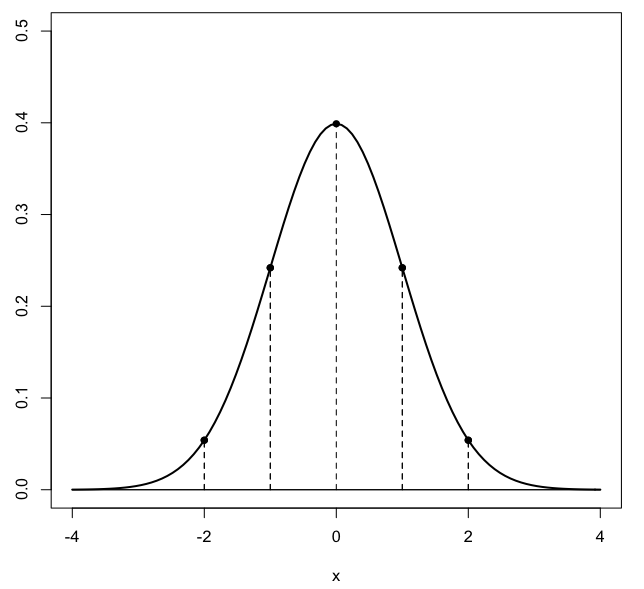
\includegraphics [scale=0.4] {gauss3.png} \end{center}

\title{Nahin}
\date{}

\begin{document}
\maketitle
\Large
\subsection*{example}

\[ f(z) = e^{-z^2} \]
Since
\[ z^2 = (x + iy)(x + iy) \]
\[ = x^2 - y^2 + 2ixy \]
We have
\[ f(z) = e^{-z^2} = e^{-x^2 + y^2 - 2ixy} \]
\[ = e^{y^2 - x^2} \ e^{i(-2xy)} \]
\[ = e^{y^2 - x^2} \ [ \ \cos -2xy + i \sin -2xy \ ] \]
\[ = e^{y^2 - x^2} \ [ \ \cos 2xy - i \sin 2xy \ ] \]
\[ = e^{y^2 - x^2} \cos 2xy - i e^{y^2 - x^2} \sin 2xy \]

Checking the CRE is a bit complicated:
\[ u = e^{y^2 - x^2} \cos 2xy \]
\[ u_x = (-2x) \  e^{y^2 - x^2} \cos 2xy -  2y \ e^{y^2 - x^2} \sin 2xy \]
\[ u_y = 2y \ e^{y^2 - x^2} \cos 2xy - 2x \ e^{y^2 - x^2} \sin 2xy \]
and
\[ v = - \ [ \ e^{y^2 - x^2} \sin 2xy \ ]  \]
\[ v_x = - \ [ \ -2x \ e^{y^2 + x^2} \sin 2xy - 2y \  e^{y^2 - x^2} \cos 2xy  \ ] \]
\[ v_y = - \ [ \ 2y \ e^{y^2 - x^2} \sin 2xy - 2x \ e^{y^2 - x^2} \cos 2xy \ ]  \]
Looks like a match.  $u_x = v_y$ and $u_y = - v_x$.

There is an important theorem that says that an analytic function $e^{w}$ of an analytic function $w = -z^2$, is itself an analytic function.  Since we won't prove this, I thought it better to check that the CRE are satisfied.

The next step Nahin carries out is to integrate this function around a particular contour:
\[ \int (u + iv) (dx + idy) \]
\[ = \int \{ u \ dx - v \ dy + i (u \ dy + v \ dx) \} \]

The path is rectangular
\begin{center} 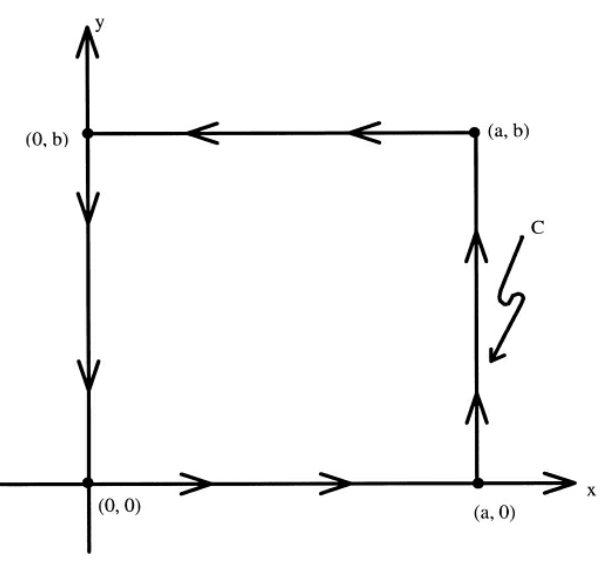
\includegraphics [scale=0.3] {nahin_path1.png} \end{center}

Cauchy does this integral at the beginning of his first, 1814, paper about complex functions.  He knows that the integral is zero (by Cauchy 1, since the function is analytic and does not blow up anywhere within the contour).

This means that both the real part and the imaginary part must be equal to zero.

We have four different parts with four different paths.  To keep this simpler, I will only do the real part.

Part 1:  $(0,0) \rightarrow (a,0)$
\[ I_1 = \int  u \ dx - \int v \ dy \]
$dy = 0$ so
\[ I_1 = \int u \ dx \]
\[ = \int_0^a e^{y^2 - x^2} \cos 2xy \ dx \]
$y = 0$ so
\[ I_1 = \int_0^a e^{- x^2} \cos 0 \ dx \]
\[ = \int_0^a e^{- x^2} \ dx  \]

Part 2: $(a,0) \rightarrow (a,b)$
\[ I_2 = \int  u \ dx - \int v \ dy \]
$dx = 0$ so
\[ I_2 = - \int_0^b v \ dy \]
\[ = - \int_0^b e^{y^2 - x^2} \sin 2xy \ dy \]
$x = a$ so
\[ I_2 = - \int_0^b e^{y^2 - a^2} \sin 2ay \ dy \]
\[ = - e^{- a^2} \int_0^b e^{y^2} \sin 2ay \ dy \]

Part 3:  $(a,b) \rightarrow (0,b)$
\[ I_3 = \int  u \ dx - \int v \ dy \]
$dy = 0$ so
\[ I_3 = \int_a^0 e^{y^2 - x^2} \cos 2xy \ dx  \]
$y = b$ so
\[ I_3 = \int_a^0 e^{b^2} \ e^{- x^2} \cos 2xb \ dx  \]
\[ = - e^{b^2} \int_0^a e^{- x^2} \cos 2xb \ dx  \]

Part 4: $(0,b) to (0,0)$
\[ I_4 = \int  u \ dx - \int v \ dy \]
$dx = 0$ so
\[ I_4 = \int - v \ dy \]
\[ = \int_b^0 e^{y^2 - x^2} \sin 2xy \ dy \]
$x = 0$ so
\[ I_4 = 0 \]

Adding together

\[ 0 =  \int_0^a e^{- x^2} \ dx - e^{- a^2} \int_0^b e^{y^2} \sin 2ay \ dy  - e^{b^2} \int_0^a e^{- x^2} \cos 2xb \ dx \]
\[  \int_0^a e^{- x^2} \ dx = e^{- a^2} \int_0^b e^{y^2} \sin 2ay \ dy  + e^{b^2} \int_0^a e^{- x^2} \cos 2xb \ dx \]

Does that look like progress?

Now, let $a \rightarrow \infty$ !!  The first term on the right-hand side goes to zero because $e^{-a^2} \rightarrow 0$ so
\[ \int_0^{\infty} e^{- x^2} \ dx = e^{-b^2} \int_0^{\infty} e^{- x^2} \cos 2xb \ dx  \]

We were supposed to already do the right-hand integral.
\[ \int_0^{\infty} e^{- x^2} \cos 2xb \ dx = \frac{\sqrt{\pi}}{2} \]

Hence:
\[ e^{-b^2}  \int_0^{\infty} e^{- x^2} \ \cos 2bx \  dx = e^{-b^2}  \ \frac{\sqrt{\pi}}{2} \]
when $b = 0$
\[ \int_0^{\infty} e^{- x^2} \  dx = \frac{\sqrt{\pi}}{2} \]

\subsection*{cleanup}


\end{document} 